\documentclass[xcolor=dvipsnames,table]{beamer}
%Ubuntu bug fix:
\definecolor{RoyalBlue}{cmyk}{1, 0.50, 0, 0}
%%%%%%%%%%%%%%%%%%%%%%%%%%%%% 
\usepackage{talk}
\usepackage{soul}
%%%%%%%%%%%%%%%%%%%%%%%%%%%
\usepackage{array}   % for \newcolumntype macro
\newcolumntype{L}{>{$}l<{$}} % math-mode version of "l" column type
\newcolumntype{R}{>{$}r<{$}} % math-mode version of "r" column type
\newcolumntype{C}{>{$}c<{$}} % math-mode version of "c" column type
\usepackage{booktabs}
%%%%%%%%%%%%%%%%%%%%%%
%\usepackage{mycolors}
\usepackage{fp}
\usepackage{tabularx}
\usepackage{multirow}
\usepackage{kbordermatrix}
% \usepackage{coloremoji}
\newcommand{\arXiv}[1]{\href{https://arxiv.org/abs/#1}{arXiv:#1}}
\widescreen

\newenvironment<>{varblock}[2][.9\textwidth]{%
  \setlength{\textwidth}{#1}
  \begin{actionenv}#3%
    \def\insertblocktitle{#2}%
    \par%
    \usebeamertemplate{block begin}}
  {\par%
    \usebeamertemplate{block end}%
  \end{actionenv}}


% set block transparency: https://tex.stackexchange.com/a/44716/59580
\addtobeamertemplate{block begin}{\pgfsetfillopacity{0.8}}{\pgfsetfillopacity{1}}
\addtobeamertemplate{block alerted begin}{\pgfsetfillopacity{0.8}}{\pgfsetfillopacity{1}}
\addtobeamertemplate{block example begin}{\pgfsetfillopacity{0.8}}{\pgfsetfillopacity{1}}


\title{Neutrino masses and dark matter}
\subtitle{Scotogenic models}


%\subtitle
%{Reconstruction of the neutrino mass matrix} % (optional)

\author{Diego Restrepo
}
% - Use the \inst{?} command only if the authors have different
%   affiliation.
\institute{
  \begin{picture}(100,2)
    \put(230,-99){ \includegraphics[scale=0.32]{logosilafae}
    }
\end{picture}
  \affiliation{\tiny Instituto de Física\\
Universidad de Antioquia\\
Phenomenology Group %\\
%\& UNICAMP
}%
{http://gfif.udea.edu.co}%
{}%
{pixel}% small image here, use pixel for nothing
{}
%\arxiv{ ... %arXiv:2112.09524 [Frontiers in Physics]  arXiv:2205.05762 [PRD]
%  arXiv:1812.05523 [PRD], 1906.09685 [PRD], 1907.11938, 1909.09574
%}
%\collaborators{Kimy Agudelo, Andrés Rivera and David Suárez (UdeA)
%}
}

\date{\tiny %December 3, 2019 - COMHEP

  %[PDF: \url{http://bit.ly/comhep2019}]
} % (optional) \today
%{
\includegraphics[scale=0.3]{udea}}
\titlegraphic{\hfill
\includegraphics[height=1.5cm]{udea}}

%\subject{Talks}
% This is only inserted into the PDF information catalog. Can be left
% out. 


% If you have a file called "university-logo-filename.xxx", where xxx
% is a graphic format that can be processed by latex or pdflatex,
% resp., then you can add a logo as follows:

% \pgfdeclareimage[height=0.5cm]{university-logo}{university-logo-filename}
% \logo{\pgfuseimage{university-logo}}



% Delete this, if you do not want the table of contents to pop up at
% the beginning of each subsection:
%\AtBeginSubsection[]
%{
%  \begin{frame}<beamer>
%    \frametitle{Outline}
%    \tableofcontents[currentsection,currentsubsection]
%  \end{frame}
%}
\setbeamercolor{block title}{bg=black!90,fg=white}

\newcommand{\chml}[2]{$\underline{\text{#1\hspace{#2}}}$}
\begin{document}


%=============== 
\begin{comentar}
%===============  
%=============
\end{comentar}
%=============

\maketitle

%\section{Model building}




%\section{}
%A model of electroweak baryogenesis requiring no fine
%tuning and consistent to scales far above 1 TeV is
%demonstrated, in which dark matter plays the leading
%role in creating a CP asymmetry that is the source of
%the baryon asymmetry.

%%%%%%%%%%%%%%%
{
  \usebackgroundtemplate{
\includegraphics[width=\paperwidth,height=10cm]{dmbernal}}

  \begin{frame}
    \vspace{6cm}
    \hfill From Nicolas Bernal at NEMO-C (Medellín 2024)
  \end{frame}
}

%%%%%%%%%%%%%%%%%%%%%%%%%
\include{evidencesila}
%%%%%%%%%%

\begin{frame}
  \frametitle{Example: Inert doublet model: \hfill \small Deshpande\&Ma'77}
  SM + Inert Higgs doublet \hfill Lopez Honorez\&\emph{et al}'06
  \begin{columns}
    \begin{column}{0.3\textwidth}

  \begin{align*}
    \eta =
    \begin{pmatrix}
      \eta^+\\
      H_0 + i A_0\\
    \end{pmatrix}
  \end{align*}

      
    \end{column}  
    \begin{column}{0.7\textwidth}


\includegraphics[scale=0.3]{idmann}
      
    \end{column}  
  \end{columns}
  


  \centering
  
\includegraphics[scale=0.25]{idmyaguna}
  
  
  
\end{frame}

{
  \usebackgroundtemplate{
\includegraphics[width=\paperwidth]{  effectivenuMD  }}%\only<2>{effectivenuMD}}}
  \begin{frame}
    \frametitle{\centering Effective neutrino masses \\
    Majorana\hfill {Dirac}}

  \vspace{1.3cm}
  
  \begin{center}
  \rowcolors{1}{RoyalBlue!20}{}
  \begin{tabular}{lcccc}
    Name & $SU(2)_L$& $U(1)_Y$ & $U(1)_L$ & $\only<1>{Z_2}\only<2>{\color{red}Z_2'}$\\
    $L$    & $\boldsymbol{2}$ & $-1/2$ & $-1$ & $\only<1>{+}\only<2>{\color{red}+}$\\
    $H$    & $\boldsymbol{2}$ & $1/2$ & $0$ & $\only<1>{+}\only<2>{\color{red}+}$\\
   \invisible<1>{ $\color{red}\nu_R$    & $\boldsymbol{1}$ & $0$ & $-1$ & $\color{red}-$\\}
  \end{tabular}
    
  \end{center}


  
  \begin{columns}
    \begin{column}{0.5\textwidth}
      \begin{align*}
   \mathcal{L}_{M} = \frac{y_M}{\Lambda}    L \cdot H L \cdot H + \text{h.c}  \to \Delta L = 2
      \end{align*}
    \end{column}
    \begin{column}{0.5\textwidth}
      \begin{align*}
   \invisible<1>{\mathcal{L}_{D} =   \cancel{y_D \left({\color{red} \nu_R}\right)^\dagger L \cdot H}  + \text{h.c}  }
      \end{align*}
    \end{column}

  \end{columns}

  \begin{center}
\only<1>{Dark matter (radiative) realization $\to Z_2$}\only<2>{Avoids Higgs mechanism for {\color{red} $\nu_R\to Z_2'$} }
  \end{center}


  \begin{columns}
    \begin{column}{0.5\textwidth}

    \end{column}
    \begin{column}{0.5\textwidth}
      \begin{align*}
       \invisible<1>{\cancel{ M_N {\color{red}\nu_R \nu_R}} \to U(1)}
      \end{align*}
    \end{column}

  \end{columns}
  
  \end{frame}
}


{
  \usebackgroundtemplate{
\includegraphics[width=\paperwidth]{topologies1}}

\begin{frame}
    \frametitle{\centering Scotogenic one-loop realizations \\
    Majorana\hfill Dirac}
\end{frame}
}

{
  \usebackgroundtemplate{
\includegraphics[width=\paperwidth]{topologies2}}

\begin{frame}
    \frametitle{\centering Scotogenic one-loop realizations \\
    Majorana\hfill Dirac}
\end{frame}
}

{
  \usebackgroundtemplate{
\includegraphics[width=\paperwidth]{scotogenic}}

\begin{frame}
    \frametitle{
    Majorana\hfill Dirac}


  \begin{columns}
    \begin{column}{0.5\textwidth}
  \begin{center}
  \rowcolors{1}{RoyalBlue!20}{}
  \begin{tabular}{lccc}
    Name & $SU(2)_L$& $U(1)_Y$& $Z_2$\\
    $\color{red}N_R$ & $\boldsymbol{1}$ & $0$ & $-$\\
    $\eta$ & $\boldsymbol{2}$ & $1/2$ & $-$\\
  \end{tabular}
   \end{center}
 \end{column}
 
 \begin{column}{0.5\textwidth}
   \vspace{-1cm}
      \begin{center}
        \rowcolors{1}{RoyalBlue!20}{}
       \begin{tabular}{lcccc}
    Name & $SU(2)_L$& $U(1)_Y$& $Z_2$ & $U(1)_L$\\
         $\nu_R$ & $\boldsymbol{1}$ & $0$ & $-$ & $-1$ \\
         $\color{red}\psi_R$ & $\boldsymbol{1}$ & $0$ & $+$ & $r-1$ \\
         $\color{red}\psi_L$ & $\boldsymbol{1}$ & $0$ & $+$ & $r-1$ \\
         $\eta$ & $\boldsymbol{2}$ & $1/2$ & $+$ & $r$\\
    $\sigma$ & $\boldsymbol{1}$ & $0$ & $-$ & $r$\\         
  \end{tabular}
\end{center}
    \end{column}

  \end{columns}


\end{frame}
}


{
  \usebackgroundtemplate{
\includegraphics[width=\paperwidth]{mediators}}

\begin{frame}
    \frametitle{ Majorana\hfill Dirac}
\end{frame}
}

{
  \usebackgroundtemplate{
\includegraphics[width=\paperwidth]{u1b-l}}

\begin{frame}
    \frametitle{ Majorana\hfill From $Z_2\times U(1)$ to local $U(1)_{B-L}$: Dirac}
\end{frame}
}





\begin{frame}
  \frametitle{From $Z_2\times U(1)$ to a (secluded) U(1) gauge symmetry with chiral fermions}
  In a fundamental theory the elementary fermions are expected to be chiral, i.e, the their charges should not allow a mass term
larger than the scale of spontaneous symmetry breaking. For
  any set of chargues associted to a U(1) gauge symmetry
\begin{align*}
  \boldsymbol{{\color{blue}Z}} = \left[Z_1,Z_2,\cdots,Z_N\right]\,,
\end{align*}
The triangle anomaly with three U(1) gauge
bosons on the external lines, i.e., the $[U(1)]^3$ anomaly, and with one
U(1) gauge boson and two gravitons on the external lines
should also be cancelled %\cite{1905.13729}

\begin{align}
    \label{eq:Dcoond}
    \sum_{\alpha=1}^{N} Z_\alpha=&0\,,&
    \sum_{\alpha=1}^{N} Z_\alpha^3=&0\,,
\end{align}
%
\end{frame}


\begin{frame}
  \frametitle{$U(1)_Y$: no vector-like,  i.e., pairs of fields with `equal-but-opposite'
charges}
  The hypercharge for one generation in the standard model can be seen as gauge Abelian symmetry $U(1)_Y$ with 15 left-handed Weyl
massless fermions with integer charges
\begin{align*}
  Y = [\color{red}1, 1,\color{blue} 1, 1, \color{Green} 1, 1, \color{red} -4, \color{blue} -4, \color{Green} \color{red}-4, 2,\color{blue} 2, \color{Green}2, \color{magenta} -3, -3, 6]
\end{align*}
which satisfy
\begin{align*}
  \sum_i Y_i =& 0\,, & \sum_i Y_i^3 =& 0\,.
\end{align*}
If we introduce an scalar, $\color{magenta}H$, of charge $\color{magenta}3$ we can form Yukawa couplings through the Dirac pairs
\begin{align*}
 u_\alpha=& \color{red}(1, -4), \color{blue}(1, -4), \color{Green}(1, -4),& d_\alpha = & \color{red}(1, 2), \color{blue}(1, 2), \color{Green}(1, 2),& e= & \color{magenta} (-3,6)
\end{align*}
and the \emph{chiral fermions} acquire Dirac masses after the EWSB. They are degenerate because the additional color symmetry. One remains massless, $\nu_L = \color{magenta} (-3)$.
The renmant $\color{magenta}Z_3$ symmetry guarantees the stability of  the lightest quark


\end{frame}



\begin{frame}
   \frametitle{Secluded gauge $U(1)_{\color{magenta}D}$  without vector-like fermions:   }
   \begin{align*}
   \boldsymbol{{\color{blue}S}} =     \left[ \chi_1,\chi_2,\cdots,\psi_{1},\psi_2,\cdots,\psi_{N'}\right]
   \end{align*}
   \vspace{-0.5cm}
   \begin{itemize}%[4,4,-5,-1,-1,-1] like with a massles protected fermion which does not thermalize
     \item \emph{\color{red}Dark Higgs mechanism}: Singlet dark Higgs $\color{Green}\phi$ acquires a vev and give mass to the dark photon
       \begin{align}
  \mathcal{L}=i \psi_{a}^{\dagger}\overline{\sigma^\mu}\left(\partial_\mu -i g_D Z^D_\mu \right)\psi_{a}-\frac{1}{4}V_{\mu\nu} V^{ \mu\nu }+\color{blue} \sum_{a<b}h_{ab} \psi_{a}\psi_b {\color{Green}\phi^{(*)}} +\text{h.c} {\color{Green}-V(\phi)}\,.
       \end{align}

   \item  $S_\alpha$  are the charges of SM-singlet right-handed chiral fermions with $N\ge 5$
     \begin{itemize}

     \item $\chi_i$ \emph{\color{red}massless fermions} with $i=1,\cdots, N'$ with $N'\le N$ 
     \item $\psi_a$ \emph{\color{red}multi-component dark matter}: massive after
       the spontaneous symmetry breaking of $U(1)_{\color{magenta}D}$
       with $a=N'+1,\cdots, N$
     \end{itemize}
   \item \emph{\color{red}Larger parameter space}:  Dark photon, $Z_D$, exclusions instead of $Z'$ 
   \item $Z_D$ and $\color{Green}\phi$ masses are related by (arXiv:1610.03063)
     \begin{align*}
       h/g_D = \sqrt{2}m_\psi /m_{Z_D}\,.
     \end{align*}
   \end{itemize}
\end{frame}


\begin{frame}
    \frametitle{\small Multi-component and two-mediator DM with kinetic mixing }


\centering

\includegraphics[scale=0.4]{dmsectors}



\end{frame}

{
  \usebackgroundtemplate{
\includegraphics[width=\paperwidth]{sltns}}

\begin{frame}
  \frametitle{\centering Two-mediator: Dark photon and dark Higgs }

  
  \begin{columns}
    \begin{column}{0.5\textwidth}

    \begin{align*}
      \begin{pmatrix}
h_1 \\
h_2
\end{pmatrix}
=
\begin{pmatrix}
\cos \alpha & -\sin \alpha \\
\sin \alpha & \cos \alpha
\end{pmatrix}
\begin{pmatrix}
\mathrm{Re}(H^0) \\
\mathrm{Re}(S)
\end{pmatrix}
    \end{align*}

    \end{column}
    \begin{column}{0.5\textwidth}
      \begin{align*}
        \mathcal{L}_{B'} \supset -\frac{\epsilon}{2}B'_{\mu\nu}B^{\mu\nu}
      \end{align*}

      \footnotesize
      \begin{align*}
        \begin{pmatrix}
          A^\mu\\
          Z^\mu\\
          {Z'}^\mu\\
        \end{pmatrix} = 
        \frac{1}{4}v^2 
\begin{pmatrix}
 g_1^2 & -g_1 g_2  & - g_1^2 \epsilon  \\
 - g_1 g_2 & g_2^2 &  g_1 g_2\epsilon  \\
 - g_1^2  \epsilon  &  g_1 g_2 \epsilon  & 324g_D^2\frac{v^2_S}{v^2}+g_1^2\epsilon ^2 \\
\end{pmatrix}
                \begin{pmatrix}
          B^\mu\\
          W^\mu_3\\
          {B'}^\mu\\
        \end{pmatrix}
      \end{align*}

    \end{column}
  \end{columns}


\end{frame}
}

\begin{frame}
 
\includegraphics[scale=0.25]{schannelZprime}   
\includegraphics[scale=0.25]{tchannelZprime}  
\includegraphics[scale=0.33]{schannelZprimeHiggs}  
\includegraphics[scale=0.25]{tchannelZprimeHiggs}  



\includegraphics[scale=0.25]{schannelscalar} 
\includegraphics[scale=0.25]{tchannelscalar}

\includegraphics[scale=0.33]{annihilation_Z_prime}

DM conversion channels


\includegraphics[scale=0.25]{conversionZprime}
\hspace{0.1cm}

\includegraphics[scale=0.25]{conversionscalar}
\end{frame}


\begin{frame}
  \frametitle{Effective Dirac neutrino mass operator \hfill \tiny{arXiv:2112.09524}}
Decrease the number of charges to be assigned to dark matter particles, $\psi_i$ below%\only<2>{}
  \begin{align*}
    \left[ \chi_1,\chi_2,\cdots,\psi_{1},\psi_2,\cdots,\psi_{N'}\right]\\
    \text{\color{cyan} Secluded case: } \\
    \left[{\color{red}\nu,\nu, (\nu)}, \psi_{1},\psi_2,\cdots,\psi_{N'} \right]
  \end{align*}
\begin{align*}
  { \color{red}  \chi_1\to \nu_{R1},\cdots, \chi_{N_\nu}\to \nu_{R\, N_\nu},\qquad 2\le N_\nu\le 3\,,}
\end{align*}
  \begin{align*} 
    \mathcal{L}_{\text{eff}} = h_{\nu}^{ij} \, {\color{red}\left( \nu_{R i}\right)^{\dagger}} \, \epsilon_{ab} \, {\color{blue} L_j^a }\,H^{b} \left(\frac{{\color{Green}\phi^*}}{\Lambda}\right)^\delta + \text{H.c.},\qquad \text{with $i,j=1,2,3$}\,,
\end{align*}
$\color{Green}\phi$ is the complex singlet scalar responsible for the SSB of the anomaly-free gauge symmetry and
\setlength{\fboxrule}{3 pt}
\fcolorbox{red}{yellow}{give mass to \emph{all} $\psi_a$}
\begin{align*}
     \label{eq:effcon}
   {\color{Green} \phi}=-\frac{\color{red}\nu}{\delta}\,,
\end{align*}

\end{frame}



\begin{frame}
  \frametitle{Effective Dirac neutrino mass operator \hfill \tiny{arXiv:2112.09524}}
Decrease the number of charges to be assigned to dark matter particles, $\psi_i$ below\only<2>{}
  \begin{align*}
    \left[ \chi_1,\chi_2,\cdots,\psi_{1},\psi_2,\cdots,\psi_{N'}\right]\\
    \text{\color{cyan} Secluded case: } \\
    \left[{\color{red}5,5}, {\color{blue} -3,-2 ,} {\color{Green}1,-6 } \right]
  \end{align*}
\begin{align*}
  { \color{red}  \chi_1\to \nu_{R\,1},\ \chi_{2}\to \nu_{R\,2},\qquad N_\nu=2\,,}
\end{align*}
  \begin{align*} 
    \mathcal{L}_{\text{eff}} = h_{\nu}^{aj} \, {\color{red}\left( \nu_{R a}\right)^{\dagger}} \, \epsilon_{bc} \, {\color{blue} L_j^b }\,H^{c} \left(\frac{{\color{Green}\phi^*}}{\Lambda}\right) + \text{H.c.},\qquad \text{with $j=1,2,3$}\,,
  \end{align*}

  \invisible<1>{
  
  \begin{align*}
  \boldsymbol{z}=[{\color{red}5,5}, {\color{blue} -3,-2 ,} {\color{Green}1,-6 }] \to {\color{Green}\phi}=-5 \to [{\color{red} (5, 5)},{\color{blue}(-3, -2)},{\color{Green}(1, -6)}] 
\end{align*}

\begin{align*}
  \setlength{\fboxrule}{3 pt}
  \mathcal{L}\subset
  {\color{blue}h_{(-3,-2)}\psi_{-3}\psi_{-2}{\color{Green}\phi^*}}
  +{\color{Green}h_{(1,-5)}\psi_1\psi_{-6}\phi^*}
  +\text{h.c.}
\end{align*}
}
\end{frame}

{
  \usebackgroundtemplate{
\includegraphics[width=\paperwidth]{sltns}}

\begin{frame}
    \frametitle{ Majorana\hfill Dirac}
  \begin{columns}
    \begin{column}{0.5\textwidth}
\vspace{-1cm}
  \begin{align*}
    \left[\psi_{1},\psi_2,\cdots,\psi_{N}\right]
  \end{align*}

        \vspace{-0.3cm}
      
\includegraphics[scale=0.6]{darkscoto}

      \vspace{-0.7cm}
  
      \begin{align*}
        \frac{y}{\Lambda} LLHH 
        \to \frac{y}{\Lambda}LLHH{{\color{Green}\frac{\phi}{\Lambda} \frac{\phi^*}{\Lambda}}}
      \end{align*}

      
  $\color{Green}\phi$ 
\setlength{\fboxrule}{3 pt}
\fcolorbox{red}{yellow}{give mass to \emph{all} $\psi_a$}
  
    \end{column}

    \begin{column}{0.5\textwidth}

\vspace{-1.5cm}
  \begin{align*}
    \left[{\color{red}\nu,\nu, (\nu)}, \psi_{1},\psi_2,\cdots,\psi_{N'} \right]
  \end{align*}

  

      \vspace{-0.3cm}
      
\includegraphics[scale=0.6]{darkscotodir}

        \vspace{-0.7cm}
      \begin{align*}
        y \left(\nu_R\right)^\dagger L H \to y \left(\nu_R\right)^\dagger L H  
        \frac{{\color{Green}\phi^*}}{\Lambda}
      \end{align*}

      
  $\color{Green}\phi$ 
\setlength{\fboxrule}{3 pt}
\fcolorbox{red}{yellow}{give mass to \emph{all} $\psi_a$}


      
    \end{column}
  \end{columns}

  

    
  \end{frame}
}



{
  \usebackgroundtemplate{
\includegraphics[width=\paperwidth]{sltnsend}}

\begin{frame}
  \frametitle{ Majorana \hspace{4cm}{\color{cyan}\small Minimal inert scalar sector.}\hfill Dirac}
  \begin{columns}
    \begin{column}{0.5\textwidth}
\vspace{-1cm}
  \begin{align*}
    \left[\psi_{1},\psi_2,\cdots,\psi_{N}\right]
  \end{align*}

        \vspace{-0.3cm}
      
\includegraphics[scale=0.6]{darkscotomaj}

      \vspace{-0.7cm}
\begin{align*}
   {\color{Green}\phi}=2 \to \big[{\color{blue}\underbrace{1,1}_{\displaystyle{\psi_a}}} ,{\color{black} (2, -4), (4, -6)},{\color{red}(3, -5)}\big] 
\end{align*}
  
  
    \end{column}

    \begin{column}{0.5\textwidth}

\vspace{-1.5cm}
  \begin{align*}
    \left[{\color{red}\nu,\nu, (\nu)}, \psi_{1},\psi_2,\cdots,\psi_{N'} \right]
  \end{align*}

  

      \vspace{-0.3cm}
      
\includegraphics[scale=0.6]{darkscotodirac}

        \vspace{-0.7cm}
\begin{align*}
  {\color{Green}\phi}=9 \to \big[
[{\color{red}9,9,9,} {\color{blue} \underbrace{(1,-10),(1,-10)}_{\displaystyle{\psi_a}},} \color{black}(-4,-5)\big],
\end{align*}


      
    \end{column}
  \end{columns}

  

    
  \end{frame}
}


{
  \usebackgroundtemplate{
\includegraphics[width=\paperwidth]{sltnsresults}}

\begin{frame}
  \frametitle{ Majorana \hspace{4cm}{\color{cyan}\small Minimal inert scalar sector.}\hfill Dirac}
  \begin{columns}
    \begin{column}{0.5\textwidth}
      \vspace{-7cm}
\begin{align*}
   {\color{Green}\phi}=2 \to \big[{\color{blue}{1,1}} ,{\color{black} (2, -4), (4, -6)},{\color{red}(3, -5)}\big] 
\end{align*}
  
Secluded DM with Majorana fermion candidate  
    \end{column}

    \begin{column}{0.5\textwidth}

      \vspace{-1cm}
\begin{align*}
  {\color{Green}\phi}=9 \to \big[
[{\color{red}9,9,9,} {\color{blue} {(1,-10),(1,-10)},} \color{black}(-4,-5)\big],
\end{align*}

New decay channel: $Z_D \to \bar{\nu}\nu $

\vspace{6cm}

In progress...
    \end{column}
  \end{columns}

  

    
  \end{frame}
}



{
  \usebackgroundtemplate{
\includegraphics[width=\paperwidth]{venues}}

\begin{frame}
\frametitle{Many other venues}
\end{frame}
}

\begin{frame}
  \frametitle{Conclusions}

  Scotogenic models, which explain dark matter and neutrino masses and mixings, have diverse realizations with a wide range of predictions through various portals and messengers.

  When applied to chiral dark matter models arising from Abelian gauge symmetries, the stability of dark matter is automatically ensured, giving rise to a rich secluded dark sector.
\end{frame}

{
%\usebackgroundtemplate{
\includegraphics[height=\paperheight]{silafaegua}}    
  \plain{
  %\only<2>{
\includegraphics[scale=0.9]{slfg}}
  
  Thanks!}
}

\end{document}



TEMPLATES

1. Background image slide
%%%%%%%%%%%%%%%%%%%%%%%%%%%%%%
{
\usebackgroundtemplate{\includegraphics[width=\paperwidth]{file}}
\setbeamertemplate{blocks}[rounded][shadow=false]
\setbeamercovered{invisible}
\begin{frame}[plain]
\end{frame}
}
%%%%%%%%%%%%%%%%%%%%%%%%%%%%%%

2. Two columns
\begin{columns}
  \begin{column}{0.48\textwidth}
    
  \end{column}
  \begin{column}{0.48\textwidth}
    
  \end{column}
\end{columns}




\begin{columns}
  \column{.48\textwidth}
  \begin{block}<2->{}
  \end{block}
  \column{.48\textwidth}
  \begin{block}<2->{}
  \end{block}
\end{columns}

%%%%%%%%%%%%%%%%%%%%%
{
\usebackgroundtemplate{\includegraphics[width=\paperwidth]{file}}
\setbeamertemplate{blocks}[rounded][shadow=false]
\setbeamercovered{invisible}
\begin{frame}[plain]
  \begin{block}{}
    Name
  \end{block}
\end{frame}
}
%%%%
{
\usebackgroundtemplate{\includegraphics[width=\paperwidth]{file}}
\setbeamertemplate{blocks}[rounded][shadow=false]
\setbeamercovered{invisible}
\begin{frame}[plain]
\end{frame}
%%%%%%%%%%%%%%%%%%
}


%Trick to put stuff in specfic places of an slide:
\begin{frame}
\begin{picture}(320,250)
\put(-25,190){D.R. \emph{et al}: arXiv:1006.5075 [PRD]\qquad\qquad arXiv:1206.3605 [PRD]}
\put(-37,20){
\includegraphics[scale=0.35]{atmcorrelationm}}
\put(143,20){
\includegraphics[scale=0.35]{LoverWlZnu_Dm23_500_500_randomm}}
\put(0,160){Only depend in \alert{$\Lambda_i$}}
\end{picture}
\end{frame}
%%%%%
Background like
%%%%%%%%%%%%%%%%%%%%%%%%
\begin{frame}[plain]
\begin{picture}(320,250)
\only<1>{\put(-30,-15){
\includegraphics[width=\paperwidth]{brpv1}}}%
\only<2>{\put(-30,-15){
\includegraphics[width=\paperwidth]{brpv2}}}%    
\only<2>{\put(-30,-15){
\includegraphics[width=\paperwidth]{brpv3}}}%    
\end{picture}
\end{frame}


%%%
Post it

\setbeamercolor{postit}{fg=black,bg=yellow}
\begin{beamercolorbox}[sep=1em,wd=5cm]{postit}
Place me somewhere!
\end{beamercolorbox}

%%%combine with textblock
\begin{textblock*}{297mm}(0mm,0mm)%
\begin{beamercolorbox}[sep=0.1em,wd=4cm,center,rounded=true,shadow=true]{cite}
\scriptsize Akhmedov, hep-ph/0001264
\end{beamercolorbox}
\end{textblock*}

%%More colorboxes
\setlength{\fboxrule}{3 pt}
\fcolorbox{red}{yellow}{caja de fondo
amarillo y contorno rojo}\\
\setlength{\fboxsep}{5pt}
\fcolorbox{red}{yellow}{caja de fondo
amarillo y contorno rojo}

\only<11>{\put(-20,80){
\begin{minipage}[t]{1.0\linewidth}
%\metroset{block=fill}
\begin{block}{SM particles}
     Gauge invariance+Lorentz Invariance$\to$Lagrangian (interactions)   
\end{block}
    \end{minipage}
}}


\begin{frame}
\begin{picture}(320,250)
\only<1->{\put(0,100){
  \begin{overpic}[scale=0.4,grid
            ]{table1}
\put(40,38){\tikz \draw[red,thick,rounded corners] (0,0) rectangle (2,0.5);}
  \end{overpic}
}
\only<1->{\put(34,158.5){ some text  }}%
\only<1->{\put(-20,140){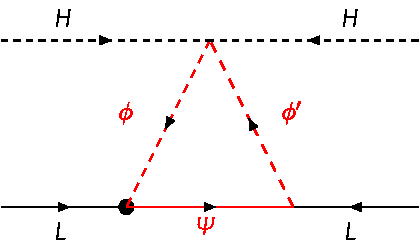
\includegraphics[scale=0.8]{T3}}}%
}
  \only<2->{\put(-10,70){
      \begin{minipage}[t]{1.0\linewidth}
      \begin{block}{ 
\includegraphics[scale=0.1]{new} Globall symmetries safe for high multiplets:}
     Catà, Ibarra, Ingenhütt arXiv:1611.00725 (PRD), arXiv:1707.08480 (JCAP)    
      \end{block}
      \end{minipage}
%
  }}
%%%circle
\end{picture}
\end{frame}


\begin{frame}
  \frametitle{Is the glass half empty or half full?}
   Tree-level SM-portal could be fully excluded in the near future

  \begin{columns}
    \begin{column}{0.5\textwidth}
      \begin{itemize}
      \item Singlet scalar dark matter
      \item Inert doublet model
      \item Tree-level SM-portal dark matter $\cdots$
      \end{itemize}
    \end{column}
    \begin{column}{0.5\textwidth}

      \only<1>{
\includegraphics[scale=0.2]{x1t} }%
      \only<2->{
\includegraphics[scale=0.3,angle=180]{halffill} }

    %\hfill  \tiny{\url{Dreamstime.com}}  
    \end{column}

  \end{columns}

  In this talk we explore
  \begin{itemize}
  \item<2-> Recover SM-portals in LR models 
  \item<3-> New portals in LR models 
  \end{itemize}

\end{frame}


Custom width in block. See definition in preamble
\begin{frame}
      \begin{varblock}[12cm]{DM is made of two color octets with mass around $12.5\ \text{TeV}$}      
      \end{varblock}
\end{frame}

Several pages frame
\begin{frame}[fragile,allowframebreaks]
  
\end{frame}
